\chapter{Instructions for officers}
This assumes you have super-user privileges.
So it contains some higher-level administration tasks.

\section{Uploading scans}
Self-explanatory, but some gotchas:
\begin{itemize}
	\ii For safety, uploaded filenames \emph{must} be distinct.
	(This is to prevent someone from accidentally submitting the form twice,
	or submitting the same PDF twice.)
	If your scanner has silly filenames, fix those.
	Also, filenames should end with either ``pdf'' or ``PDF''.

	\ii At the moment we don't have image processing,
	so please make sure all scans are correctly rotated.

	\ii \emph{Please}, make sure you are uploading the scans
	to the correct contest!
	There are some ways to deal with such mistakes but better
	if they can be avoided in the first place.
\end{itemize}

\begin{center}
	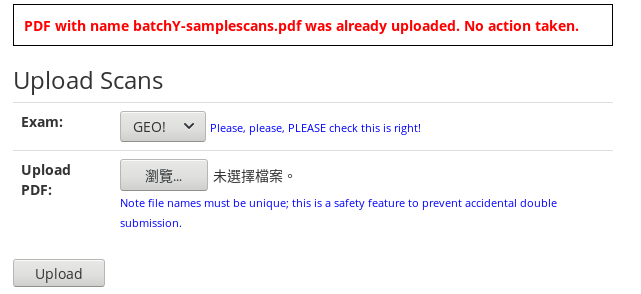
\includegraphics[width=0.8\textwidth]{images/batchscan.png}
\end{center}

When you upload a scan,
several problem scribbles, exam scribbles, and verdicts
are immediately created corresponding to the items in the PDF file.
However since the system does not yet know who is who,
the verdicts and problem scribbles will not have an entity attached to them.
The ``match scans'' functionality will then pair them up.

It seems preferable to upload scans in smaller batches,
rather than all at once.
This way, after the first PDF is uploaded,
graders can start marking immediately
while future PDF's are uploaded.

\section{Matching scans}
Matching scans is more error-prone and not double-checked.
People who should do this should be ones who are a little familiar with
all the teams attending and so on (e.g.\ TD's and registration director at HMMT).

\begin{center}
	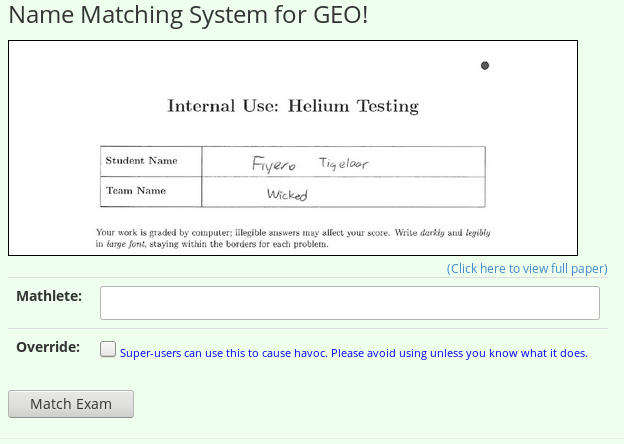
\includegraphics[width=0.8\textwidth]{images/papermatch.png}
\end{center}

Interface usage: a name will be shown.
\begin{itemize}
	\ii Find the corresponding entity, and submit.
	\ii If all goes well, next entity will be shown.
\end{itemize}
Easy.
When a match of a paper is successful,
all the problem scribbles, exam scribbles, and verdicts
attached to the paper are immediately updated to reflect the new name.

The comments in Section~\ref{sec:view_full} apply equally well here.

\subsection{Error handling}
This is where it gets tricky.
Consider the following situation:
\begin{quote}
	You match a geometry exam to a student ``Christine Daae''.  
	Later on, you try to match another geometry exam
	to the same student ``Christine Daae''.
\end{quote}
This is obviously not okay, and the system will complain.
An error will appear linking to the first \emph{verdict}
it finds for a geometry problem taken by Christine Daae.

\begin{center}
	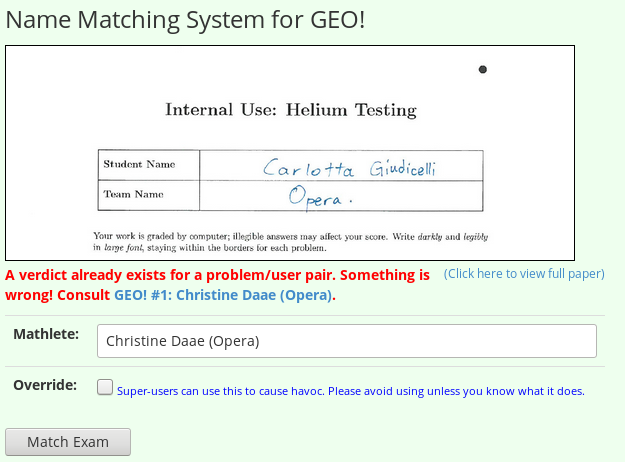
\includegraphics[width=0.7\textwidth]{images/matchconflict.png}
\end{center}

At this point you need to fix the error.
There are a couple things you could do.
\begin{itemize}
	\ii If you made the mistake this time,
	then just re-submit the form with the correct name. Easy.

	\ii If you made the mistake the \emph{first} time around,
	then you need to go back and fix it.

	You can do this by clicking on the verdict provided by the system,
	and then opening the exam scribble for that verdict.
	Alternatively, the ``Find Papers'' interface will let you find
	the previous paper as well.
	This will bring you to a match form where you can change the
	name to the correct one.

	\ii As a last resort,
	the ``Override'' switch (visible only to super-users)
	will forcibly assign the paper,
	and retroactively delete all verdicts and
	problems scribbles to the contrary.
	This is a Bad Idea\texttrademark\ and you should only do it
	if you really understand Helium well and have a compelling reason to do so.
\end{itemize}

\section{Find papers}
You can locate specific papers
by selecting ``Find Papers'' from the index page.
Some ways to do so:
\begin{itemize}
	\ii You can look up by exam and entity.
	\ii You can scroll through the pages of the PDF files.
	\ii A list of papers which need moderator attention
	will appear here (see Section~\ref{sec:view_full}).
\end{itemize}

\begin{center}
	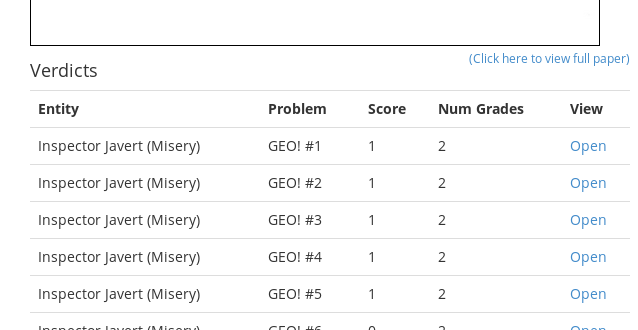
\includegraphics[width=0.6\textwidth]{images/viewpaper2.png}
\end{center}

If the paper has an exam scribble associated,
that will also be displayed,
along with a form to change the name associated to it
(in case of error).

\begin{center}
	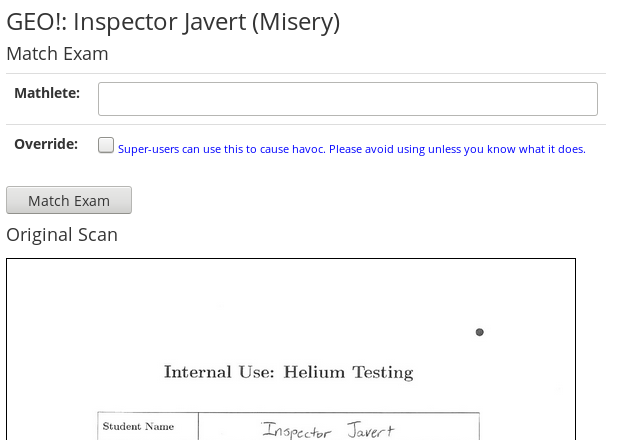
\includegraphics[width=0.6\textwidth]{images/viewpaper1.png}
\end{center}

\section{Conflict resolution}
First, I should describe the logic behind verdicts.
For each exam there are two parameters:
\begin{itemize}
	\ii A \textbf{minimum majority} for the verdict to be valid,
	defined as a constant $n$ such that an $n$-to-$1$ majority suffices.
	\ii If valid, a \textbf{minimum number of graders} needed before
	the verdict considers itself done.
	(So setting this number to $2$ is double-grading,
	$3$ is triple-grading, etc.\ and the default is $3$.)
\end{itemize}

Officers get an extra panel called ``View All Conflicts''.
This lets you see the grading conflicts for \emph{everyone}.

\begin{center}
	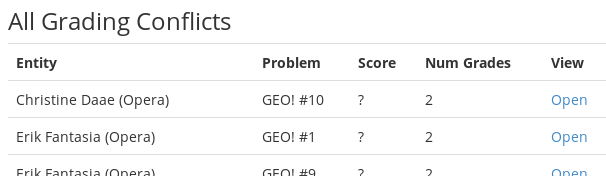
\includegraphics[width=0.8\textwidth]{images/all-conflict.png}
\end{center}

Given a conflict, you can open the verdict page corresponding to it,
at which point you can submit your own evidence.
If you like being final authority,
there should also be an option to submit this evidence in ``God mode''
which will settle the verdict once and for all.
\section{Finishing results}
Once grading is all said and done,
you can download the results at the bottom of the page.
Administrators can also download full results
and a full score spreadsheet.

Note that algorithmic scoring is not done automatically,
since it is a long and intensive operation.
To run it, you should use the management command
``Run Algorithmic Scoring'',
after all verdicts are settled.
Alternatively (and maybe better), you can use
\verb+python manage.py algscore+ from SSH.

\section{Other Administration}
The Django admin interface can be used if there
is some operation you need to do not supported by the existing views.

\subsection{Management}
In addition, to operations that might be useful
but in theory should not be necessary:
\begin{itemize}
	\ii ``Compute Verdicts'' will ask every verdict (and there will be many!)
	to re-compute its judgment.
	Normally, verdicts only re-compute their judgment when they get new evidence.
	This is needed if e.g.\ you change the thresholds for grading.

	\ii ``Update scribbles'' is similar,
	it updates all problem scribbles and verdicts
	with matched names.
	This should basically never be necessary unless you done goof.
\end{itemize}
Both of these commands actually just run \verb+manage.py+ commands,
so they can also be done from SSH.

\subsection{Someone uploaded PDF to wrong exam!}
Well, that's a bummer.  You should
\begin{itemize}
	\ii Delete the relevant PDF file from the Django admin interface.
	This will kill of the exam and problem scribbles too.
	\ii Delete all the verdicts that no have neither an entity or problem scribble.
\end{itemize}
That should mostly save things. No priomises though.
